\documentclass{article}

\usepackage[affil-it]{authblk}
\usepackage{graphicx}
\usepackage{float}
\usepackage[ruled]{algorithm2e}
\usepackage{titlepic}
\usepackage{multicol}
\usepackage{chngcntr}

\counterwithin{figure}{section}
\graphicspath{{../resources/}}

\SetKwProg{function}{Function}{}{end}
\newcommand{\assign}[2]{$#1 \leftarrow$ #2}

\title{COMP390 Evolving a Sorting Algorithm with SNGP}
\author{Robin Lockyer\\{\small Student ID: 201148882 \\ Primary Supervisor: Dr. David Jackson \\ Secondary Supervisor: Dr. Valentina Tamma}}
\date{2018/2019}
\titlepic{\includegraphics[width=0.5\textwidth]{UOL_Logo.png}}

\begin{document}
	
	\maketitle	
	
	\newpage
	
	\begin{abstract}
		
		Genetic programming is a technique for creating programmes not by writing them by hand, but instead by creating a population of random programmes and modifying them using an evolutionary algorithm. The desired result is that after several generations a programme that performs well at a given task is generated. GP has previously been used to successfully evolve sorting algorithms.
		
		Single node genetic programming is a variation on GP invented by Dr Jackson which structures the population of programmes in a manner that allows the use of dynamic programming when computing the result of the programmes in an effort to more efficiently generate a working solution. 
		
		This project aims to compare the effectiveness of the two methods in evolving a sorting algorithm.
		
	\end{abstract}
	\newpage
	\tableofcontents
	\newpage
	\section{Introduction}
	
        This project is was done for my project supervisor Dr David Jackson. The aim of this project is to attempt to evolve a sorting algorithm using node genetic programming (SNGP) and, if successful, compare the effectiveness of evolving sorting algorithms using standard genetic programming (GP) to evolving sorts with SNGP.
        
        The purpose of GP is to automate the creation of algorithms and programmes. This is done by applying a genetic algorithm to a population of random programmes so that successive generations of programmes improve at the desired characteristics until a functional programme is created.
        The standard approach to GP requires evaluating hundreds of programmes per generation over potentially thousands of generations and as such GP can take up a large amount of processing time. Several variations of GP have been created that try to reduce the amount of processing, including Linear Genetic Programming and Parallel Distributed GP \cite{poli_field_2008}.
        
        SNGP is one such variation devised by Dr Jackson in \textit{A New, Node-Focused Model for Genetic Programming} \cite{jackson_new_2012}. This variation makes use of a form of dynamic programming to re-use results of previously evaluated programmes. It has been shown that SNGP tends to perform better than standard GP in terms of processing time, solution rate, and solution size \cite{jackson_new_2012}. SNGP has reduced efficiency when dealing with problems with side-effects because this prevents re-use of evaluations, although it still performs better than GP at some problems with side effects \cite{jackson_single_2012}. 
        
        A sorting algorithm reads and manipulates an array of integers as it executes, and so must make use of side effects. Regular genetic programming has been shown to be capable of evolving a working sorting algorithm \cite{kinnear_evolving_1993,kinnear_generality_1993}. This makes evolving a sort a good problem to evaluate SNGP on as comparisons can be made with previous research.
        
	\section{Background}
	
    \subsection{Standard Genetic Programming}\label{Section:GP}
        
        Genetic programming allows the user to automate finding solutions to problems without the need to know much about the solutions themselves. This is done by a stochastic process where successive generations of programmes are altered to create the next generation, with the goal of each generation being an improvement on the last until a desired result is found.
        
        In standard the standard form of GP, described in \textit{A Field Guide to Genetic programming} \cite{poli_field_2008}, programmes are encoded as a tree of primitive functions and terminals. Each function has a number of child nodes equal to it's arity, and each individual child represents a single operand of the parent function. Nodes with no children represent terminal functions or constants which require no input. Figure \ref{fig:ex_prog_tree} shows an example of a programme encoded as a tree.
        
        \begin{figure}
            \centering
            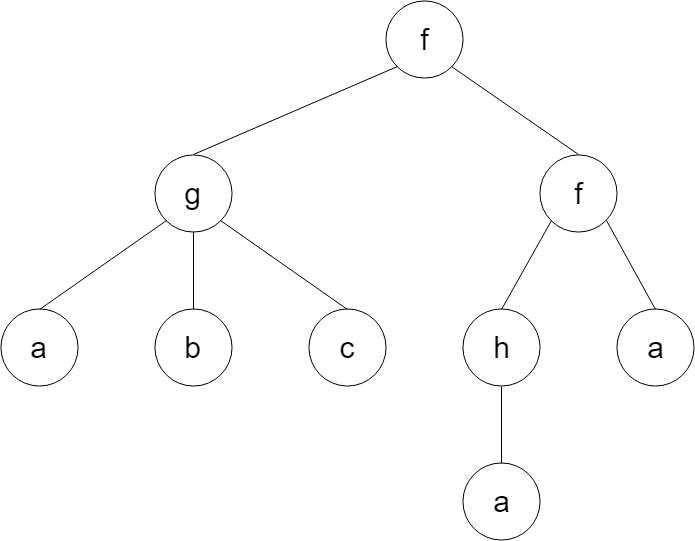
\includegraphics[width=0.5\textwidth]{1_gp_example_tree}
            \caption{This tree encodes the programme f( g( a, b, c ), f( h( a ), a ) ), where f, g, and h are functions and a, b, and c are terminals.}
            \label{fig:ex_prog_tree}
        \end{figure}
        
        An initial population of random programme trees is generated according to certain parameters that can vary depending on implementation. Each member of the population is executed in turn. The results of these executions are evaluated and each member of the population is given a fitness score so that better programmes have higher scores.
        
        Members of the population are then selected to produce offspring programs based on their fitness. Simply selecting the best individuals to reproduce can lead to low diversity in the resulting population, so a probabilistic is often used to prevent a single programme's offspring from dominating subsequent generations.
        Common methods for doing this include fitness proportionate selection, where the probability of selection is proportional to the fitness of the individual relative to the fitness of the whole population, and tournament selection, where a small subset of programmes are chosen with equal probability and the fittest of the subset is selected for reproduction.
        
        Genetic operators are then applied to the chosen programmes to create a new generation. The operator selected to create each member is chosen with a pre selected probability. The three most commonly used operators, which are also the three operators Koza used to successfully evolve a sort \cite{kinnear_evolving_1993}, are:
        
        \begin{itemize}
            \item \textbf{Reproduction:} 
            
            \begin{figure}[h]
                \centering
                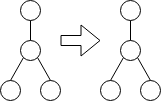
\includegraphics[width=0.3\textwidth]{5_reproduction}
                \caption{Example of reproduction operator}
                \label{fig:reproduction}
            \end{figure}
            
            The selected programme is copied into the new generation without modification. Reproduction tends to have a low selection probability to ensure the following generation si sufficiently different.
            
            \item \textbf{Crossover:} 
            
            \begin{figure}[h]
                \centering
                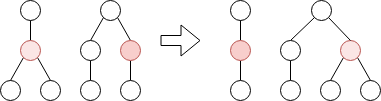
\includegraphics[height=0.2\textwidth]{6_crossover}
                \caption{Example of crossover operation. The highlighted nodes are the crossover points}
                \label{fig:crossover}
            \end{figure}
            
            A random node is selected as the crossover point in each of the two chosen programmes and the subtrees rooted at the selected nodes are swapped.
            
            
            \item \textbf{Mutation:} 
            
            \begin{figure}[h]
                \centering
                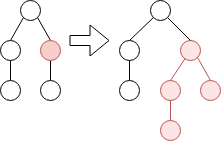
\includegraphics[width=0.4\textwidth]{7_mutation}
                \caption{Example of mutation operator. The highlighted node is replaced by the highlighted subtree.}
                \label{fig:mutation}
            \end{figure}
            
            A random node is selected in the chosen programme. A new, random subtree is generated to replace the subtree rooted at the selected node.
        \end{itemize}
        
        The process of creating new generation is continued until a certain condition is reached, usually after a certain number of generations or a programme exceeds a fitness specified by the user.
        
        Genetic programming has been previously been shown to evolve a sorting algorithm by Kenneth E Kinnear \cite{kinnear_generality_1993,kinnear_evolving_1993}. hIS work was not focused on evolving an optimal sort, but instead attempting to see if GP was capable of evolving any kind of sort at all. Kinnear considered sorting to be an interesting problem to solve using GP as there are many possible ways to implement a sorting algorithm, and the domain of the problem is infinite.
        
	\subsection{Single Node Genetic Programming}
	
        Single Node Genetic Programming is a variant of GP that uses a form of dynamic programming to speed up the evaluation of GP programmes.
        
        The population is organised a single directed acyclic graph. This allows the nodes to be organised into a topological ordering such that any given node only uses nodes later in the ordering as operands. The nodes are stored in an array in this order, with all the terminals occupying the lowest values, as shown in Figure \ref{fig:sngp_graph}.
        
        \begin{figure}[h]
            \centering
            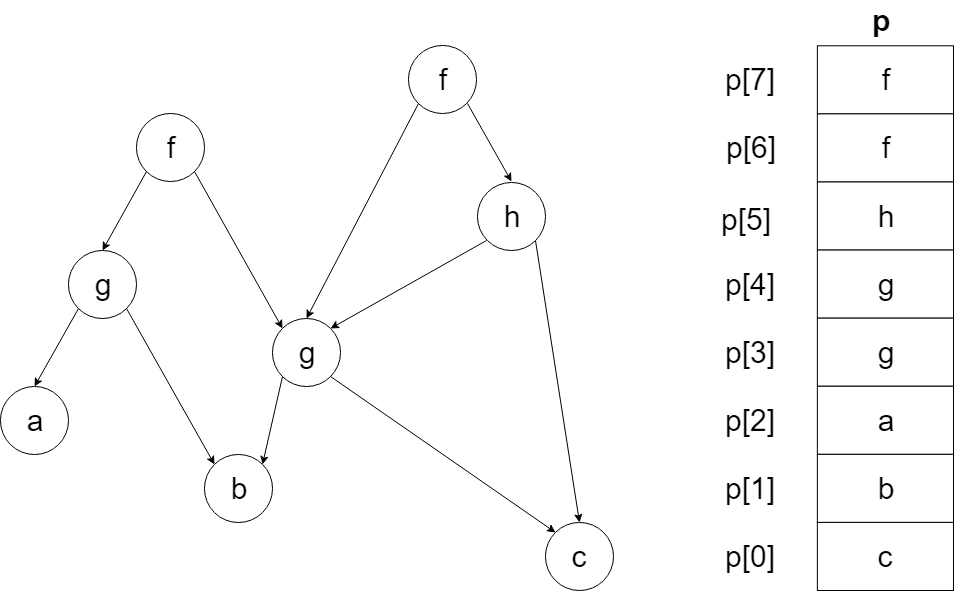
\includegraphics[width=0.5\textwidth]{8_sngp_graph}
            \caption{This SNGP graph is stored in topological order in an array. Terminals a,b, and c occupy the lowest positions of the array.}
            \label{fig:sngp_graph}
        \end{figure}
        
        Every subtree within the graph represents a single programme. For example the graph in Figure \ref{fig:sngp_graph} contains the following programmes:
        
        \begin{multicols}{2}
            \begin{itemize}
                \item a
                \item b
                \item c
                \item g( b, c )
                \item g( a, b )
                \item h( g( b, c ), c )
                \item f( g( a, b ), g( b, c ) )
                \item f( g( b, c ), h( g( b, c ), c ) )
            \end{itemize}
        \end{multicols}
        
        This allows many different programmes to be represented in a single graph as each node is itself a programme, while in regular GP there are many nodes per programme. The structure also allows for sharing of subtrees between programmes so that if there exists a programme with a particularly high fitness, other programmes can make use of the same subtrees to improve their fitness.
        
        Evaluation of the population starts from the subtree rooted at the lowest element of the array and works upwards. The results of each evaluation are saved and can be re-used whenever the subtree needs to be executed as part of a larger programme, making the evaluation of an SNGP population very efficient.
        
        SNGP uses only one genetic operator called \textit{successor mutate}. This operator picks a random function node in the graph and changes an operand with another random node with a lower index in the population array. Instead of the whole population being re-evaluated only the the modified node and programmes that make use of that node need to be evaluated. These nodes can be determined by keeping track of the parents of each node and using this information backtrack up the graph from the modified node. When backtracking to determine which nodes to update it is important to visit nodes in array order to ensure that subtrees are updated before their results are re-used.
        
        \begin{figure}[h]
            \centering
            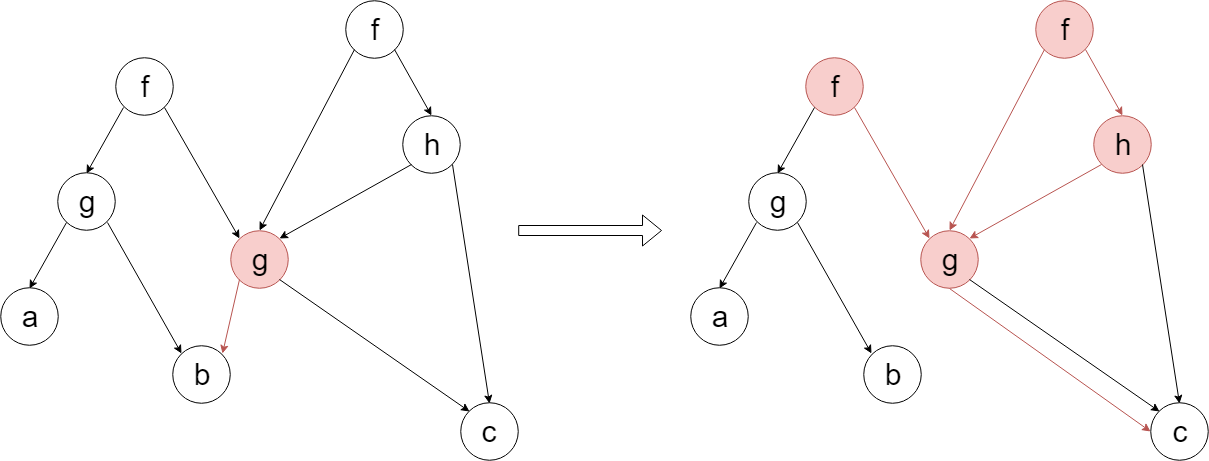
\includegraphics[width=0.5\textwidth]{10_successor_mutate}
            \caption{A successor mutate operation is applied to the highlighted node on the left graph, resulting in the right graph. Highlighted nodes on the left graph should be re-evaluated}
            \label{fig:successor_mut}
        \end{figure}
        
        Successor mutate allows for the modification of many programmes with a single genetic operator, and the modification itself is very efficient. Evaluation of the new population tend to be more efficient than in GP as SNGP can make use of the prior evaluation from the unchanged subtrees from the previous generation.
        
        After application of the successor mutate operator the population as a whole is given a fitness value. If the application has improved the fitness value then the change is kept, otherwise the change is reverted. There are variation of SNGP that differ in how to assign a fitness to the population:
        
        \begin{itemize}
            \item \textbf{SNGP/A:} The population fitness is the average fitness of the whole population.
            
            \item \textbf{SNGP/B:} The population fitness is the fitness of the best individual within the population.
        \end{itemize} 
        
        Like GP, this process is repeated for a certain number of generations or a programme exceeds a fitness specified by the user.
        
        SNGP has been shown to produce a working solutions after fewer generations than GP, as well as producing many more working solutions in the same number of generations \cite{jackson_new_2012}. The programmes produced tend to be smaller than those in GP, most likely due to the maximum size of any programme being capped by the size of the population, and the re-use of subtrees within a single programme.
        
        SNGP cannot make use of dynamic programming when dealing with primitives with side effects. The result of a subtree may differ depending on what is executed beforehand, so the subtree must be executed again for each other programme that makes use of it. However, even with this disadvantage SNGP/B still requires fewer evaluations to find a solution than GP in some cases, although this is dependant on the specific problem being solved \cite{jackson_single_2012}.
        
	\section{Design and Realisation}
	
	\subsection{GP Implementation}
	
        The GP implementation was based example code given by Dr Jackson and also on an implementation of the TinyGP system found in the book \textit{A Field Guide to Genetic
            Programming} \cite{poli_field_2008}. It was written in C as the example code given to me was also in C. The parameters are the same as described in Koza's work \cite{kinnear_generality_1993}.
        
        Each programme is stored as a string of primitive functions and terminals. The string is in prefix notation, and as all primitives have fixed arity no bracketing is needed. Programmes also store their fitness and their size. The information is stored as a struct, detailed in Figure \ref{struct:gp_prog}.
        
        \begin{figure}[h]
            \centering
            \begin{tabular}{|l l|}
                \hline
                \multicolumn{2}{|c|}{Prog}\\
                \hline
                Primitive[] & code \\
                double & fitness\\
                int & proglen\\
                \hline
            \end{tabular}
            \caption{Data structure to store a programme. The \textit{code} array stores a string representing the prefix notation of the programme tree, \textit{fitness} stores the programmes fitness, and \textit{proglen} the number of nodes in the programme tree.}
            
            \label{struct:gp_prog}
        \end{figure}
        
        The primitives used for this implementation are the same nine Kinnear used:
        \begin{multicols}{2}
            \begin{itemize}
                \item \textbf{INDEX:} A terminal that gives the current index of the ITERATE function.
                \item \textbf{LENGTH:} A terminal that gives the length of the current array.
                \item \textbf{ITERATE(start, end, function):}  Sets index to the value of start and increments index by one until index equals end or index equals length -1. Each iteration will execute function a single time. This primitive will return the minimum of end and LENGTH. To prevent excessive execution time, programmes are capped at 10000 total iterations.
                \item \textbf{SWAP(x,y):}  Swaps the elements of the array at positions x and y. Returns x.
                \item \textbf{SMALLEST(x,y):} Compares the values of the array at x and y. Returns the index of the smaller.
                \item \textbf{LARGEST(x,y):} Compares the values of the array at x and y. Returns the index of the larger. 
                
                \item \textbf{SUBTRACT(x,y):} Returns the value of x – y.
                \item \textbf{INCREMENT(x):} Returns the value of x+1.
                \item \textbf{DECREMENT(x):} Returns the value of x-1.
                
            \end{itemize}
        \end{multicols}
        
        The primitives are defined in an enumeration, and a table is kept to store the names and arities of the primitives. An additional \textit{DUMMY} primitive is also included to occupy the 0 value of the enumeration and make all actual primitives have arity > 0. This is useful when debugging and in certain algorithms for identifying when a primitive has not been assigned. These data structures are shown in Figure \ref{struct:arity}.
        
        \begin{figure}[h]
            \centering
            
            enum Primitive = $\left \{p1,p2,…,pn-1,pn \right\}$
            
            \smallskip
            
            \begin{tabular}{|l l|}
                \hline
                \multicolumn{2}{|c|}{TableEntry}\\
                \hline
                Primitive & primitive \\
                int & arity\\
                char[] & name\\
                \hline
            \end{tabular}
            
            \bigskip
            
            TableEntry[] arityTable = $\left\{\left \{ p1,0,"PrimitiveName"\right\},…,\left\{ pn,k,"PrimitiveName"\right\}\right\}$
            
            \caption{Data structures used to store information about primitives}
            
            \label{struct:arity}
        \end{figure}
        
        The each member of the population is initialised by using the grow method. A maximum tree depth is specified and a random primitive is selected as the root. Random primitives are selected as the children for primitives that have been previously selected. The primitives can be either functions or terminals, unless selecting a function would cause the tree to exceed the maximum depth. The initial maximum depth is chosen to be 6 to match Koza's work. The pseudocode for the algorithm is shown in algorithm \ref{alg:createTree}.
        
        \begin{algorithm}
            \SetKw{createTree}{createTree}
            
            
            \function{\createTree{$(maxDepth)$}:}{
                
                
                
                \uIf{$maxTreeDepth = 1$}{
                    
                    \KwOut{$randomTerminal()$}
                    
                }
                \Else{elseif-block}{
                    
                    \assign{root}{$randomPrimitive()$}
                    
                    \For{\assign{i}{1} to $arityTable[root].arity$}{
                        
                        \assign{root.operand[i]}{\createTree{$(maxDepth-1)$}}
                        
                    }
                    
                    \KwOut{root}
                    
                }
            }
            
            \label{alg:createTree}
            \caption{Algorithm to initialise a programme as a random tree with a given depth}
        \end{algorithm}

        Three genetic operators used are the three mentioned in section \ref{Section:GP}. Crossover is used to generate 80\% of the next generation, and 20\% is generated by reproduction. There is also a 10\% change that mutation will be applied to each member of the new population. The pseudocode for this is shown in algorithm \ref{alg:GP}.

        \begin{algorithm}[H]
            
            $initialisePopulation()$
            
            $evaluatePopulation(0)$
            
            \For{$generation \leftarrow 1$ \KwTo $NUM\_GENERATIONS$}{
                
                \For{$j \leftarrow$  \KwTo $POPULATION\_SIZE$}{
                    
                    \uIf{$randInt(1,10) <= 8$}{
                        
                        $newPopulation[j] \leftarrow crossover(selectProg(),selectProg())$
                        
                    }
                    \Else{$newPopulation[j] \leftarrow reproduce(selectProg())$ }
                    
                }
                
                \ForEach{$programme \in newPopulation$}{
                    
                    \If{$randInt(1,10) = 1$}{
                        
                        $mutate(programme)$
                        
                    }
                    
                }
                
                $population \leftarrow newPopulation$
                
                $evaluatePopulation(generation)$
                
            }
            
            \KwOut{$best(population)$}
            
            \caption{Genetic Programming Algorithm}
            
            \label{alg:GP}
        \end{algorithm}
    
    	\bigskip
    
    	The three genetic operators use the following algorithms:
    	
    	\begin{algorithm}[H]
    		
    		\KwIn{parentProg}
    		
    		\KwOut{parentProg}
    		
    		\caption{Reproduction Operator}
    		
    		\label{alg:reproduction}
    		
    	\end{algorithm}
    
    	\begin{algorithm}[H]
    		
    		\KwIn{parentProg1}
    		\KwIn{parentProg2}
    		
    		\assign{crossoverPoint1}{$randInt(1,parent1.proglen)$}
    		\assign{crossoverPoint2}{$randInt(1,parent2.proglen)$}
    		
    		\assign{childProg1}{$replaceSubtree( parentProg1, crossoverPoint1, parentProg2.prog[crossoverPoint2] )$}
    		
    		\assign{childProg2}{$replaceSubtree( parentProg2, crossoverPoint2, parentProg1.prog[crossoverPoint1] )$}
    		
    		\KwOut{childProg1}
    		\KwOut{childProg2}
    		
    		\caption{Crossover Operator}
    		
    		\label{alg:crossover}
    		
    	\end{algorithm}
    
    	\begin{algorithm}[H]
    		
    		\KwIn{parentProg}
    		
    		\assign{randomNode}{$randInt(1,parentProg.proglen)$}
    		
    		\assign{childProg}{$replaceSubtree( parentProg, randomNode, randomTree() )$}
    		
    		\KwOut{childProg}
    		
    		\caption{Mutation Operator}
    		
    		\label{alg:mutation}
    		
    	\end{algorithm}
    
    	

	\subsection{SNGP Implementation}
        
        The SNGP implementation was solely based on Dr Jackson example code. Much of it was re-used from my GP implementation, including the primitives and arity table.
        
        Each node in the SNGP population stores its current fitness, fitness from th previous generation, an array of operands, an array of predecessors, and the number of nodes in the programme tree. This is stored in the data structure shown in figure \ref{struct:sngp_node}. An arity table is also stored in the same was as in GP.
        
        \begin{figure}[H]
            \centering
            \begin{tabular}{|l l|}
                \hline
                \multicolumn{2}{|c|}{Node}\\
                \hline
                Primitive & primitive \\
                double & fitness\\
                double & oldFitness\\
                int[] & operands\\
                iny[] & predecessors\\
                int & proglen\\
                \hline
            \end{tabular}
            \caption{Data structure to store information about each node in the SNGP population}
            
            \label{struct:sngp_node}
        \end{figure}
        
        The array of predecessors is a fixed length, the same as the population array. It stores the indicies of each predecessor in a linked list, where $predecessor[0]$ contains the value of the predecessor with the smallest index, $p_1$, and then $predecessor[p_1]$ stores the value of the next largest predecessor, $p_2$, and so on until $predecessor[p_n] = 0$. This method allows for efficient traversal, insertion, and deletion, while using a fixed amount of memory.
        
        \begin{figure}[h]
        	
        	\centering
        	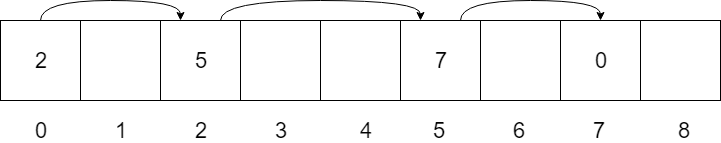
\includegraphics[width=0.5\textwidth]{predecessor_array}
        	\caption{A predecessor array containing the indices 2, 5, and 7}
        	\caption{fig:predecessor}
        	
        \end{figure}
    
    	This structure is used again to determine which nodes should be updated after performing a successor mutate operation.
    	
    	\begin{algorithm}[h]
    		
    		\SetKw{buildUpdateList}{buildUpdateList}
    		\SetKw{addToUpdateList}{addToUpdateList}
    		
    		\function{\buildUpdateList{$(mutatedNodeIndex)$}:}{
    			
    			$addToUpdateList(mutatedNodeIndex)$
    				
    			\assign{predecessors}{$population[mutatedNodeIndex].predecessors$}
    			
    			\assign{nextPredecessorIndex}{$predecessors[0]$}
    			
    			\While{$\lnot(nextPredecessorIndex = 0)$}{
    			
    				\assign{inList}{addToUpdateList($nextPredecessorIndex)$}
    				
    				\If{$inList$}{
    				
    					$buildUpdateList(nextPredecessorIndex)$
    			
    				}
    			
    				\assign{nextPredecessorIndex}{$predecessors[nextPredecessorIndex]$}
    		
    			}
    			
    		}
    		\function{\addToUpdateList{$(nodeIndex)$}:}{
    			
    			\assign{nextValue}{$0$}
    				
    			\While{$\lnot(updateList[nextValue] = 0)\land updateList[nextValue] < nodeIndex$ }{
    			
    				\assign{nextValue}{$updateList[nextValue]$}
    				
    			}
    		
    			\uIf{$\lnot(updateList[nextValue] = nodeIndex)$}{
    			
    				\assign{updateList[nodeIndex]}{$updateList[nextValue]$}
    				\assign{updateList[nextValue]}{$nodeIndex$}
    				
    				\KwOut{False}
    		
    			}
    			\Else{\KwOut{True}}
    	
    		}
    		
    		\caption{Create list of nodes to be updated}
    		\label{alg:updateList}
    		
    	\end{algorithm}
        
        The pseudocode for the overall SNGP algorithm is:
        
        \begin{algorithm}
        	
        	
        	
        \end{algorithm}
	
	\subsection{Fitness Functions}
	
        While many different fitness functions were used, they all counted the number of inversions in a test array before and after executing a programme. To efficiently count inversions I used a modified merge sort algorithms, detailed in algorithm \ref{alg:countInv}. The algorithm is $O(n\log{}n)$, and merging is done using two preallocated buffers to avoid unnecessary memory allocations while the GP algorithm is running.
        
        \begin{algorithm}
            
            \SetKw{countInversions}{countInversions}
            
            \function{\countInversions{$(arr)$}:}{
                
                \uIf{$length(arr) <= 1$}{
                    
                    \assign{inversions}{$0$}
                    
                }
                
                \Else{
                    
                    \assign{sizeA}{$\left\lfloor length(arr) / 2 \right\rfloor$}
                    
                    \assign{sizeB}{length(arr) - sizeA}
                    
                    \assign{A}{[First sizeA elements of arr]}
                    
                    \assign{B}{[Last sizeB elements of arr]}
                    
                    \assign{inversions}{countInversions(A) + countInversions(B)}
                    
                    \assign{C}{Empty Array}
                    
                    \While{$length(A) > 0 and length(B) > 0$}{
                        
                        \uIf{$B[1] < A[1]$}{
                            
                            Append B[1] to C
                            
                            \assign{inversions}{inversions + length(A)}
                            
                            Remove first element of B
                            
                        }
                        \Else{
                            
                            Append A[1] to C
                            
                            Remove first element of A
                            
                        }
                    }
                    
                    \uIf{$length(A) = 0$}{
                        
                        Append remaining elements of B to C
                        
                    }
                    \ElseIf{$length(B) = 0$}{
                        Append remaining elements of A to C
                    }
                    
                    \assign{arr}{C}
                    
                }
                
                \KwOut{inversions}
                
            }
            
            \caption{Algorithm that sorts array and counts number of inversions}
            
            
            
            \label{alg:countInv}
            
        \end{algorithm}
        
        The fitness function I used as a starting point for both my GP and SNGP implementations was the same Kinnear used in \cite{kinnear_evolving_1993,kinnear_generality_1993}. The function is defined as the following:
        
        \begin{figure}[h]
            $$fitness(prog) = \frac{adjusted(prog)}{\sum_{p\in population}^{}adjusted(p)}$$
            
            $$adjusted(prog) = \frac{1}{1 + raw(prog)}$$
            
            $$raw(prog) = praw(prog) - \min_{p\in population} praw(p)$$
            
            $$praw(prog) = \left(\sum_{t = 1}^{Number Of Tests}res(t)\right) \cdot of + size(prog) \cdot sf$$
            
            $$res(t) = rdis(t) + pdis(t)$$
            
            $$pdis(t) = max(rdis(t) - idis(t), 0) \cdot 100$$
            
            \caption{Kinnear's Fitness Function}
            
            \label{kinnear_fitness}		
        
        \end{figure}
        Where $rdis(t)$ is the remaining number of inversions in a test array t after running a member of the population, $idis(t)$ is the initial number of inversions in a test array t, and $of$ and $sf$ are constant weights used to adjust the resulting fitness.

    \subsection{Test Data}
        
        Each programme generated during a GP run or an SNGP run is executed on a set of test arrays. This data comes from pre-generated file containing a series of random arrays loaded into the programme at the beginning of execution. This has the advantage of allowing for reproduction of results, easier testing of the programme, and prevents random number generation from increasing the execution time.
        
        The arrays are organised into fixed size groupings. Each programme in the same GP generation is executed on the same group of arrays. This was done so that each programme was subjected to the same conditions in each generation, while still preventing over fitting to a fixed set of data. This method also allows each group to be customized to meet certain requirements (e.g. contains a sorted array, a reversed array, or a very short array), but this was found to be unnecessary.
        
        The file is a standard text file where the first two values on each line are the length and number of inversions of the array, followed by the array itself. Each value is separated by a space. A blank line indicates the end of the current group of arrays.
        
        When loaded into the programme, the test arrays are stored as the following struct:
        
        \begin{figure}[h]
            \centering
            \begin{tabular}{|l l|}
                \hline
                \multicolumn{2}{|c|}{Array}\\
                \hline
                int & size \\
                int & inversions\\
                int[] & arr\\
                \hline
            \end{tabular}
            \caption{Data structure to store each test array}
            
            \label{struct:array}
        \end{figure}

    \section{Results}

        I was successful in replicating Kinnear's work in evolving a sorting algorithm using standard GP, and found his methods able to evolve a sort very easily with no modification. Figure \ref{graph:gp_success} shows 
    \section{Evaluation}

    \section{Learning Points}

    \section{Professional Issues and Data Required}

    \section{Bibliography}

    \bibliographystyle{acm}
    \bibliography{library}

    \section{Appendices}

\end{document}